\PassOptionsToPackage{table,svgnames,dvipsnames}{xcolor}
\documentclass[11pt,a4paper]{article}

% ---------- packages ----------
\usepackage[utf8]{inputenc}
\usepackage[T1]{fontenc}
\usepackage{lmodern}
\usepackage[margin=2.3cm]{geometry}
\usepackage{amsmath,amssymb,amsthm}
\usepackage{xcolor}
\usepackage[most]{tcolorbox}
\usepackage{graphicx}
\usepackage{booktabs}
\usepackage{colortbl}
\usepackage{array}
\usepackage{enumitem}
\usepackage{microtype}
\usepackage{listings}
\usepackage{fancyhdr}
\usepackage{titlesec}
\usepackage{tikz}
\usetikzlibrary{arrows.meta,positioning,shapes.geometric}
\usepackage[colorlinks=true,linkcolor=cblue,urlcolor=cteal,citecolor=cgrape]{hyperref}

% ---------- colours ----------
\definecolor{cblue}{HTML}{2563EB}
\definecolor{cteal}{HTML}{0D9488}
\definecolor{camber}{HTML}{CA8A04}
\definecolor{cred}{HTML}{DC2626}
\definecolor{cgray}{HTML}{475569}
\definecolor{cgrape}{HTML}{7C3AED}
\definecolor{ccyan}{HTML}{0891B2}
\definecolor{cpink}{HTML}{DB2777}
\definecolor{cgreen}{HTML}{16A34A}
\definecolor{corange}{HTML}{EA580C}
\definecolor{cink}{HTML}{16202E}
\definecolor{codebg}{HTML}{FBF7EE}
\definecolor{rowt}{HTML}{EFF4FF}

% ---------- section styling ----------
\titleformat{\section}[hang]
  {\color{cblue}\Large\bfseries}{\color{corange}\thesection}{0.6em}{}[{\color{cblue!30}\titlerule[1.1pt]}]
\titleformat{\subsection}{\color{cink}\large\bfseries}{\color{cteal}\thesubsection}{0.6em}{}
\titleformat{\subsubsection}{\color{cgray}\normalsize\bfseries}{\color{cgrape}\thesubsubsection}{0.6em}{}

% ---------- header/footer ----------
\setlength{\headheight}{22pt}
\addtolength{\topmargin}{-10pt}
\pagestyle{fancy}\fancyhf{}
\renewcommand{\headrulewidth}{0.8pt}
\renewcommand{\headrule}{\hbox to\headwidth{\color{cblue!40}\leaders\hrule height \headrulewidth\hfill}}
\fancyhead[L]{\small\color{cblue}\bfseries Organizing Panel Data Methods}
\fancyhead[R]{\small\color{cgray}\leftmark}
\fancyfoot[L]{\small\color{cgray} Dr Merwan Roudane}
\fancyfoot[R]{\small\color{cgray}\thepage}
\renewcommand{\sectionmark}[1]{\markboth{#1}{}}

% ---------- boxes ----------
\newtcolorbox{idea}[1][The idea]{breakable,colback=cblue!6,colframe=cblue,coltitle=white,
  fonttitle=\bfseries\small,title={#1},boxrule=0.8pt,arc=3pt,left=6pt,right=6pt,top=4pt,bottom=4pt}
\newtcolorbox{whenbox}[1][When to use it]{breakable,colback=cgreen!6,colframe=cgreen,coltitle=white,
  fonttitle=\bfseries\small,title={#1},boxrule=0.8pt,arc=3pt,left=6pt,right=6pt,top=4pt,bottom=4pt}
\newtcolorbox{avoidbox}[1][When NOT to use it]{breakable,colback=cred!5,colframe=cred,coltitle=white,
  fonttitle=\bfseries\small,title={#1},boxrule=0.8pt,arc=3pt,left=6pt,right=6pt,top=4pt,bottom=4pt}
\newtcolorbox{begbox}[1][For beginners]{breakable,colback=cteal!7,colframe=cteal,coltitle=white,
  fonttitle=\bfseries\small,title={#1},boxrule=0.8pt,arc=3pt,left=6pt,right=6pt,top=4pt,bottom=4pt}
\newtcolorbox{cmpbox}[1][The difference]{breakable,colback=camber!8,colframe=camber,coltitle=white,
  fonttitle=\bfseries\small,title={#1},boxrule=0.8pt,arc=3pt,left=6pt,right=6pt,top=4pt,bottom=4pt}
\newtcolorbox{eqbox}[1][]{colback=ccyan!6,colframe=ccyan,boxrule=0.8pt,arc=3pt,
  left=6pt,right=6pt,top=3pt,bottom=3pt,title={#1},coltitle=white,fonttitle=\bfseries\small}

% ---------- listings ----------
\lstdefinelanguage{StataL}{
  morekeywords={xtset,webuse,regress,xtreg,xtpmg,xtmg,xtdcce2,xtcd2,xtcse2,xtunitroot,
    xtpkpss,xtpqroot,xtlmbreak,xtpcointegwe,xtpcointegboot,xtbreakcoint,xtccecoint,
    xtcadfcoint,xtnonlincoint,xtbreakmodel,xtcbc,xtkpybreak,xtbfkbreak,xtquantilebreak,
    xtdynestimb,xtpvarcoint,xtgets,xtfmg,xtpfardl,xtpcaus,xtabond,xtdpdsys},
  sensitive=true, morecomment=[l]{*}, morecomment=[l]{//}, morestring=[b]",
}
\lstset{language=StataL,basicstyle=\ttfamily\footnotesize\color{cink},
  backgroundcolor=\color{codebg},keywordstyle=\color{cblue}\bfseries,
  commentstyle=\color{cteal}\itshape,stringstyle=\color{camber},
  frame=single,framesep=5pt,rulecolor=\color{cgray!35},xleftmargin=6pt,
  breaklines=true,showstringspaces=false,columns=fullflexible,aboveskip=6pt,belowskip=6pt}

% ---------- shortcuts ----------
\newcommand{\cmd}[1]{\texttt{\textcolor{corange}{#1}}}
\newcommand{\hlt}[2]{\textcolor{#1}{\textbf{#2}}}
\newcommand{\bbeta}{\boldsymbol{\beta}}
\newcommand{\btheta}{\boldsymbol{\theta}}
\newcommand{\bgamma}{\boldsymbol{\gamma}}
\newcommand{\bx}{\mathbf{x}}
\newcommand{\bff}{\mathbf{f}}
\newcommand{\bz}{\mathbf{z}}
\newcommand{\bdelta}{\boldsymbol{\delta}}
\newcommand{\bphi}{\boldsymbol{\phi}}
\newcommand{\blambda}{\boldsymbol{\lambda}}
\newcommand{\Ito}{I(1)}
\newcommand{\Izero}{I(0)}
\newcommand{\YES}{\textcolor{cgreen}{\textbf{yes}}}
\newcommand{\NO}{\textcolor{cred}{\textbf{no}}}

\begin{document}

% ======================= TITLE =======================
\begin{titlepage}\thispagestyle{empty}\centering
\vspace*{1.4cm}
{\color{cblue}\Huge\bfseries Organizing Panel Data Methods\par}
\vspace{0.4cm}{\color{corange}\rule{0.55\linewidth}{2pt}}\par\vspace{0.4cm}
{\color{cink}\LARGE From Homogeneous Slopes to Cross-Sectional\\[4pt] Dependence and Structural Breaks\par}
\vspace{0.5cm}
{\color{cteal}\large A Map of the Whole Field --- for Beginners\par}
\vspace{1.2cm}

\begin{tcolorbox}[width=0.86\linewidth,colback=cblue!5,colframe=cblue,arc=6pt,
  title={\bfseries The purpose of these notes},coltitle=white,fonttitle=\bfseries]
Most courses teach panel methods as a \emph{list}. This is a \textbf{map}. Every method here
exists because it \textbf{relaxed one assumption} of the method before it. Once you see the chain
--- Pooled $\to$ FE $\to$ MG $\to$ PMG $\to$ CCE $\to$ breaks $\to$ the frontier --- you can place
any new paper on it, and you can \emph{choose} rather than guess.\\[4pt]
Each method gets the same four questions: \hlt{cblue}{What is the idea?}
\hlt{cgreen}{When do I use it?} \hlt{cred}{When must I not?}
\hlt{camber}{How does it differ from its neighbour?}
\end{tcolorbox}

\vspace{1.2cm}
{\large\bfseries\color{cgrape} Dr Merwan Roudane\par}
{\color{cgray} Author of the \texttt{xt*} panel structural-break Stata suite (100+ modules)\par}
{\color{cgray}\small ideas.repec.org/f/pro1421 \quad$\cdot$\quad github.com/merwanroudane\par}
\vfill
{\color{cgray}\small Lecture notes: estimators, tests, comparisons, and a decision map}
\end{titlepage}

\tableofcontents
\newpage

% ======================= THE MAP =======================
\section{The map: how every method connects}
\markboth{The map}{}

\begin{idea}[Read this page first]
There is \textbf{one} idea behind the whole field. Start with the most restrictive model
imaginable, then relax \textbf{one assumption at a time}. Each relaxation buys realism and costs
parameters. Every method in this document is one step on that chain.
\end{idea}

\begin{center}
\begin{tikzpicture}[node distance=6mm and 4mm,
  box/.style={rectangle,rounded corners=3pt,draw,thick,align=center,
              minimum height=8mm,text width=30mm,font=\footnotesize\bfseries},
  lbl/.style={font=\scriptsize\itshape,text=cgray},
  ar/.style={-{Stealth[length=2.4mm]},thick,cgray}]
\node[box,fill=cgray!12,draw=cgray]      (p)  {Pooled OLS};
\node[box,fill=cblue!12,draw=cblue,below=of p]   (fe) {Fixed Effects};
\node[box,fill=cteal!12,draw=cteal,below=of fe]  (mg) {MG / PMG};
\node[box,fill=ccyan!12,draw=ccyan,below=of mg]  (cce){CCE / PANIC};
\node[box,fill=camber!14,draw=camber,below=of cce](br){Breaks};
\node[box,fill=cgrape!12,draw=cgrape,below=of br](fr) {Frontier};
\draw[ar] (p)--(fe)  node[lbl,midway,right=1mm]{+ unit heterogeneity ($\alpha_i$)};
\draw[ar] (fe)--(mg) node[lbl,midway,right=1mm]{+ slope heterogeneity ($\bbeta_i$)};
\draw[ar] (mg)--(cce)node[lbl,midway,right=1mm]{+ cross-sectional dependence ($\bff_t$)};
\draw[ar] (cce)--(br)node[lbl,midway,right=1mm]{+ parameters change over time ($\bbeta(t)$)};
\draw[ar] (br)--(fr) node[lbl,midway,right=1mm]{+ groups, per-coefficient, I(1) factors};
\end{tikzpicture}
\end{center}

\subsection{The five questions that decide everything}
\begin{center}
\rowcolors{2}{rowt}{white}
\begin{tabular}{@{}>{\bfseries}p{0.5cm} p{7.6cm} p{7.2cm}@{}}
\rowcolor{cblue}\color{white}\# & \color{white}Question & \color{white}If the answer is ``yes'' you must move to\\
1 & Do units have their own \textbf{intercepts}? & Fixed Effects (Section~2)\\
2 & Do units have their own \textbf{slopes}? & MG / PMG (Section~3)\\
3 & Do units share \textbf{common shocks}? & CCE / PANIC (Section~5)\\
4 & Are the series \textbf{non-stationary}? & unit-root \& cointegration tests (Section~6)\\
5 & Do the parameters \textbf{change over time}? & structural-break methods (Sections~7--8)\\
\end{tabular}
\rowcolors{1}{}{}
\end{center}

\begin{begbox}
Notice these are \emph{cumulative}, not alternatives. A frontier method like \cmd{xtkpybreak}
answers \textbf{all five} at once: unit effects, heterogeneous slopes, common (even \Ito) factors,
non-stationarity, and breaks. That is why it looks complicated --- it is five ideas stacked.
\end{begbox}

% ======================= HOMOGENEOUS =======================
\section{The homogeneous world}

\subsection{Pooled OLS --- the starting point}
\begin{eqbox}[Pooled OLS]
\[ y_{it}=\alpha+\bx_{it}'\bbeta+\varepsilon_{it} \]
\end{eqbox}
\begin{idea}
Ignore that the data is a panel. Treat all $NT$ observations as one big cross-section: everyone
shares the same intercept $\alpha$ and the same slope $\bbeta$.
\end{idea}
\begin{whenbox}
Only when there is genuinely \textbf{no unobserved unit-specific heterogeneity} --- or when it is
uncorrelated with $\bx$ \emph{and} you do not care about efficiency. In practice: as a
\textbf{benchmark} to compare against, almost never as the final model.
\end{whenbox}
\begin{avoidbox}
Whenever $\alpha_i$ exists and correlates with $\bx_{it}$ --- which is the normal case. Then
pooled OLS suffers \textbf{omitted-variable bias}: the estimated slope mixes the within-unit
relationship with the between-unit one, and can even have the \emph{wrong sign}.
\end{avoidbox}

\subsection{Fixed Effects --- letting intercepts differ}
\begin{eqbox}[Fixed Effects: the within transformation]
\[ y_{it}=\alpha_i+\bx_{it}'\bbeta+\varepsilon_{it}
\quad\Longrightarrow\quad
\ddot y_{it}=\ddot\bx_{it}'\bbeta+\ddot\varepsilon_{it},\qquad \ddot y_{it}=y_{it}-\bar y_{i\cdot} \]
\end{eqbox}
\begin{idea}
Subtract each unit's own time-mean. Anything constant within a unit --- including $\alpha_i$ ---
vanishes. What is left is the \textbf{within-unit} relationship.
\end{idea}
\begin{whenbox}
When you believe $\alpha_i$ is correlated with $\bx_{it}$ (the usual case) and your question is
about \textbf{within-unit} variation: ``when a country's $x$ rises, what happens to \emph{its} $y$?''
\end{whenbox}
\begin{avoidbox}
When you need coefficients on \textbf{time-invariant} regressors --- FE wipes them out. And in
\textbf{dynamic} models with small $T$: the within transformation correlates $y_{i,t-1}$ with the
demeaned error, giving \textbf{Nickell bias} of order $1/T$.
\end{avoidbox}

\subsection{Random Effects and the Hausman test}
\begin{eqbox}[Random Effects]
\[ y_{it}=\alpha+\bx_{it}'\bbeta+\underbrace{u_i+\varepsilon_{it}}_{\text{composite error}},
\qquad \mathrm{Cov}(u_i,\bx_{it})=0 \]
\end{eqbox}
RE treats $u_i$ as \emph{random} and estimates by GLS (quasi-demeaning with
$\theta=1-\sqrt{\sigma_\varepsilon^2/(T\sigma_u^2+\sigma_\varepsilon^2)}$).

\begin{cmpbox}[FE vs RE --- the only real question]
Both estimate the same $\bbeta$. The difference is a single assumption:
\textbf{is $\alpha_i$ correlated with $\bx_{it}$?}
\begin{itemize}[leftmargin=1.2em,itemsep=0pt]
 \item \hlt{cgreen}{Not correlated} $\Rightarrow$ RE is \emph{consistent and more efficient}, and can
 estimate time-invariant regressors.
 \item \hlt{cred}{Correlated} $\Rightarrow$ RE is \emph{inconsistent}; FE is still consistent.
\end{itemize}
The \textbf{Hausman test} compares them:
\[ H=(\hat\bbeta_{FE}-\hat\bbeta_{RE})'\big[V(\hat\bbeta_{FE})-V(\hat\bbeta_{RE})\big]^{-1}
(\hat\bbeta_{FE}-\hat\bbeta_{RE})\xrightarrow{d}\chi^2_K \]
$H_0$: RE is consistent. \textbf{Reject $\Rightarrow$ use FE.}
\end{cmpbox}

\begin{avoidbox}[The modern caveat on Hausman]
The classic Hausman test assumes \textbf{homogeneous slopes} and \textbf{no cross-sectional
dependence}. In macro panels both usually fail --- which is exactly why the rest of this document
exists. Do not let a Hausman test be the end of your specification search.
\end{avoidbox}

\subsection{Comparing the homogeneous family}
\begin{center}
\rowcolors{2}{rowt}{white}
\begin{tabular}{@{}>{\bfseries}l l l c l@{}}
\rowcolor{cblue}\color{white}Estimator & \color{white}Assumes about $\alpha_i$ & \color{white}Slope &
\color{white}Time-inv.\ $x$? & \color{white}Main risk\\
Pooled OLS & none ($\alpha_i=\alpha$) & common & \YES & omitted heterogeneity\\
Fixed Effects & parameter, may correlate & common & \NO & loses time-invariant vars\\
Random Effects & random, uncorrelated & common & \YES & inconsistent if assumption fails\\
Between & (uses unit means) & common & \YES & discards within variation\\
\end{tabular}
\rowcolors{1}{}{}
\end{center}

% ======================= HETEROGENEOUS =======================
\section{Slope heterogeneity: MG, PMG, DFE}

\begin{idea}[The assumption we now drop]
So far $\bbeta$ was \textbf{the same for every unit}. In a panel of countries that is a strong
claim: does a 1\% rise in energy use really raise GDP by the same amount in Norway and in Chad?
Now we let $\bbeta_i$ differ:
\[ y_{it}=\alpha_i+\bx_{it}'\bbeta_i+\varepsilon_{it} \]
\end{idea}

\subsection{Mean Group (MG) --- Pesaran \& Smith (1995)}
\begin{eqbox}[Mean Group]
\[ \hat\bbeta_{MG}=\frac1N\sum_{i=1}^{N}\hat\bbeta_i,\qquad
\widehat{V}(\hat\bbeta_{MG})=\frac{1}{N(N-1)}\sum_{i=1}^{N}(\hat\bbeta_i-\hat\bbeta_{MG})
(\hat\bbeta_i-\hat\bbeta_{MG})' \]
\end{eqbox}
\begin{idea}
Run a \textbf{separate regression for each unit}, then simply \textbf{average} the slopes. The
variance comes from how much the unit slopes \emph{disagree}.
\end{idea}
\begin{whenbox}
When slopes are genuinely heterogeneous and \textbf{$T$ is large enough} to estimate each unit's
regression on its own (rule of thumb $T\gtrsim 20$--30). It is fully flexible: it assumes nothing
about how slopes relate.
\end{whenbox}
\begin{avoidbox}
When $T$ is small --- each $\hat\bbeta_i$ is then noise, and averaging noise gives an imprecise
(though still unbiased) mean. Also sensitive to \textbf{outlier units}: one crazy country can move
the average.
\end{avoidbox}

\subsection{Pooled Mean Group (PMG) --- Pesaran, Shin \& Smith (1999)}
\begin{eqbox}[PMG: an error-correction model with a pooled long run]
\[ \Delta y_{it}=\phi_i\Big(y_{i,t-1}-\btheta'\bx_{i,t-1}\Big)
+\sum_{j}\lambda_{ij}\Delta y_{i,t-j}+\sum_{j}\bdelta_{ij}'\Delta\bx_{i,t-j}+\varepsilon_{it} \]
\end{eqbox}
\begin{idea}
A \textbf{compromise}. Notice $\btheta$ has \emph{no} $i$ subscript but $\phi_i$ and the short-run
terms do: the \hlt{cred}{long-run relationship is forced to be the same} for all units, while the
\hlt{cgreen}{speed of adjustment and short-run dynamics are free}.
\end{idea}
\begin{begbox}[Why this compromise is so popular]
Economic theory usually predicts a \textbf{common long run} (a shared equilibrium: PPP, a
production function, an energy--growth elasticity) but says nothing about how fast each country
gets there. PMG encodes exactly that belief --- and by pooling the long run it gains a lot of
efficiency over MG.
\end{begbox}
\begin{whenbox}
When theory suggests a \textbf{common long-run relationship} but heterogeneous adjustment ---
and the poolability restriction is \textbf{not rejected} by a Hausman test.
\end{whenbox}
\begin{avoidbox}
When the long-run homogeneity restriction is \textbf{false}: PMG is then inconsistent. Always test
it (below). Also note $\phi_i<0$ is required for a meaningful error-correction interpretation.
\end{avoidbox}

\subsection{Dynamic Fixed Effects (DFE)}
\begin{idea}
Pool \textbf{everything} except the intercepts: long run, short run, and adjustment speed are all
common. The most restrictive dynamic option.
\end{idea}
\begin{avoidbox}
Badly biased when slopes truly differ (Pesaran--Smith show heterogeneity bias does \emph{not}
disappear as $T\to\infty$ in dynamic models). Use it as a \textbf{benchmark}, rarely as the answer.
\end{avoidbox}

\subsection{The comparison you must know: MG vs PMG vs DFE}
\begin{center}
\rowcolors{2}{rowt}{white}
\begin{tabular}{@{}>{\bfseries}l c c c@{}}
\rowcolor{cteal}\color{white}What is pooled? & \color{white}MG & \color{white}PMG & \color{white}DFE\\
Intercepts $\alpha_i$        & free & free & free\\
\textbf{Long-run} $\btheta$  & \textcolor{cgreen}{free} & \textcolor{cred}{\textbf{pooled}} & \textcolor{cred}{\textbf{pooled}}\\
Adjustment speed $\phi_i$    & free & \textcolor{cgreen}{free} & \textcolor{cred}{pooled}\\
Short-run dynamics           & free & \textcolor{cgreen}{free} & \textcolor{cred}{pooled}\\
\midrule
Consistent if slopes differ? & \YES & only if LR is truly common & \NO\\
Efficiency                   & lowest & \textbf{middle} & highest (if true)\\
Needs large $T$?             & \YES\ (per unit) & moderate & moderate\\
Stata                        & \cmd{xtmg} & \cmd{xtpmg, pmg} & \cmd{xtpmg, dfe}\\
\end{tabular}
\rowcolors{1}{}{}
\end{center}

\begin{cmpbox}[How to choose between MG and PMG --- the Hausman poolability test]
Under long-run homogeneity \textbf{both} MG and PMG are consistent but PMG is \emph{efficient};
under heterogeneity \textbf{only MG} is consistent. That is exactly the Hausman setup:
\[ H=(\hat\btheta_{MG}-\hat\btheta_{PMG})'\big[V(\hat\btheta_{MG})-V(\hat\btheta_{PMG})\big]^{-1}
(\hat\btheta_{MG}-\hat\btheta_{PMG})\xrightarrow{d}\chi^2 \]
$H_0$: the long run is poolable. \hlt{cgreen}{Do not reject} $\Rightarrow$ report \textbf{PMG}
(more efficient). \hlt{cred}{Reject} $\Rightarrow$ report \textbf{MG}.
\end{cmpbox}

\begin{lstlisting}
xtset id year
xtpmg d.y d.x, lr(l.y l.x) ec(ec) replace pmg      // pooled long run
estimates store pmg
xtpmg d.y d.x, lr(l.y l.x) ec(ec) replace mg       // fully heterogeneous
estimates store mg
hausman mg pmg, sigmamore                          // H0: long run is poolable
\end{lstlisting}

% ======================= DYNAMICS =======================
\section{A note on dynamics: why FE breaks down}

\begin{eqbox}[The dynamic panel and Nickell bias]
\[ y_{it}=\rho y_{i,t-1}+\bx_{it}'\bbeta+\alpha_i+\varepsilon_{it},
\qquad \mathrm{Bias}(\hat\rho_{FE})=O\!\left(\frac1T\right) \]
\end{eqbox}
\begin{idea}
The within transformation subtracts $\bar y_{i\cdot}$, which \emph{contains} $\varepsilon_{it}$.
So the demeaned regressor $\ddot y_{i,t-1}$ is correlated with the demeaned error by construction.
The bias is $O(1/T)$ --- it vanishes only as $T\to\infty$.
\end{idea}
\begin{center}
\rowcolors{2}{rowt}{white}
\begin{tabular}{@{}>{\bfseries}l p{9.4cm} l@{}}
\rowcolor{corange}\color{white}Situation & \color{white}Use & \color{white}Stata\\
Small $T$, large $N$ & \textbf{GMM}: Arellano--Bond (difference), Blundell--Bond (system) & \cmd{xtabond}, \cmd{xtdpdsys}\\
Large $T$ & MG / PMG (bias is small) & \cmd{xtpmg}, \cmd{xtmg}\\
Large $T$ + dependence & dynamic CCE / CS-ARDL & \cmd{xtdcce2}\\
Dependence + \textbf{breaks} & robust dynamic estimators & \cmd{xtdynestimb}\\
\end{tabular}
\rowcolors{1}{}{}
\end{center}

% ======================= CSD =======================
\section{Cross-sectional dependence: the great divide}

\begin{idea}[The assumption we now drop]
Every method so far assumed units are \textbf{independent}. They are not: oil shocks, crises and
technology hit everyone. Model it with a \textbf{common factor} error:
\[ y_{it}=\bx_{it}'\bbeta_i+u_{it},\qquad u_{it}=\bgamma_i'\bff_t+\varepsilon_{it} \]
$\bff_t$ = unobserved global shocks; $\bgamma_i$ = how exposed unit $i$ is.
\end{idea}

\begin{avoidbox}[What happens if you ignore it]
Pooled/FE/MG standard errors are wrong and tests \textbf{over-reject}: with a shared factor there
is far \emph{less} independent information than $N$, but the formulas divide by $N$ anyway. You
will ``find'' relationships that are artefacts of the common shock.
\end{avoidbox}

\subsection{Step 1: test for it}
\begin{eqbox}[Pesaran CD test]
\[ CD=\sqrt{\frac{2T}{N(N-1)}}\sum_{i<j}\hat\rho_{ij}\ \xrightarrow{d}\ N(0,1) \]
\end{eqbox}
\begin{center}
\rowcolors{2}{rowt}{white}
\begin{tabular}{@{}>{\bfseries}l p{6.0cm} p{5.2cm}@{}}
\rowcolor{ccyan}\color{white}Test & \color{white}Valid when & \color{white}Weakness\\
Breusch--Pagan LM & \textbf{small} $N$, large $T$ & explodes for large $N$\\
Scaled LM & $N,T$ large & size distortion if $N\gg T$\\
Bias-corrected LM & large $N,T$ (FE) & needs the FE structure\\
\textbf{Pesaran CD} & \textbf{large} $N$, any $T$ & signed average can cancel out\\
CD$^*$ & large $N$ (de-factored residuals) & needs $\hat r$\\
Frees / Friedman & small--moderate $N$ & non-parametric, lower power\\
$\alpha$ exponent & measures \emph{strength}, not a test & --\\
\end{tabular}
\rowcolors{1}{}{}
\end{center}

\begin{begbox}[Classic vs modern question]
\emph{Classic:} ``is there dependence --- yes or no?''\quad
\emph{Modern:} ``\textbf{how strong} is it?'', indexed by $\alpha$ in $\sum_i|\gamma_i|=O(N^\alpha)$:
$\alpha=1$ \hlt{cred}{strong} (a real factor $\Rightarrow$ CCE/PANIC);
$\tfrac12<\alpha<1$ \hlt{camber}{semi-weak}; $\alpha\le\tfrac12$ \hlt{cgreen}{weak/spatial}
(robust s.e.\ may suffice).
\end{begbox}

\subsection{Step 2: remove it --- the two families}
\subsubsection{Family A: cross-sectional averages (CCE)}
\begin{eqbox}[CCE --- Pesaran (2006)]
\[ \hat\bbeta_i=(X_i'\bar M X_i)^{-1}X_i'\bar M y_i,\qquad
\bar M=I-\bar Z(\bar Z'\bar Z)^{-1}\bar Z',\quad \bar Z=[\bar y,\bar X] \]
\[ \hat\bbeta_{CCEMG}=\frac1N\sum_i\hat\bbeta_i \qquad\text{(Mean Group)};\qquad
\hat\bbeta_{CCEP}\ \text{(Pooled)} \]
\end{eqbox}
\begin{idea}
\textbf{Do not estimate the factors.} Their footprint is already in the cross-section averages
$\bar y_t,\bar\bx_t$ --- so add those as regressors and project them out. You never need to know
\emph{how many} factors there are.
\end{idea}
\begin{whenbox}
The default in modern macro panels. Especially when you want \textbf{heterogeneous slopes}, do not
want to commit to a number of factors, and --- crucially --- when the factors may be \textbf{\Ito}
(Kapetanios--Pesaran--Yamagata 2011 prove CCE survives this).
\end{whenbox}
\begin{avoidbox}
When $N$ is small (the averages are noisy), or the \textbf{rank condition} fails
($\mathrm{rank}(\bar\Gamma)=r\le k+1$: you need at least as many observables as factors).
\end{avoidbox}

\paragraph{The CCE family tree.}
\begin{center}
\rowcolors{2}{rowt}{white}
\begin{tabular}{@{}>{\bfseries}l p{9.6cm} l@{}}
\rowcolor{ccyan}\color{white}Member & \color{white}What it adds & \color{white}Reference\\
CCEMG & averages the unit slopes; heterogeneous & Pesaran (2006)\\
CCEP & pools the slopes; efficient if homogeneous & Pesaran (2006)\\
Dynamic CCE & extra lags of the averages (needed if dynamic) & Chudik--Pesaran (2015)\\
CS-ARDL & dynamics + averages; long run \emph{and} short run & Chudik et al.\\
CS-DL & estimates the long run \emph{directly}, robust to lag misspecification & Chudik et al.\\
F-CCEMG & + unit-specific \textbf{Fourier} terms $\Rightarrow$ absorbs heterogeneously-timed breaks & Guliyev (2026)\\
CCE + break & + a \textbf{common} structural break (and \Ito\ factors) & BFK; KPY; BFW\\
\end{tabular}
\rowcolors{1}{}{}
\end{center}

\subsubsection{Family B: principal components (PANIC / IFE)}
\begin{eqbox}[PANIC --- Bai \& Ng (2004)]
\[ \Delta y_{it}=\bgamma_i'\Delta\bff_t+\Delta e_{it}\ \xrightarrow{\ \text{PCA on differences}\ }\
\hat\bff_t=\sum_{s\le t}\Delta\hat\bff_s,\quad \hat e_{it}=\sum_{s\le t}\Delta\hat e_{is} \]
\end{eqbox}
\begin{idea}
\textbf{Estimate the factors explicitly}. You cannot run PCA on levels when $\bff_t$ and $e_{it}$
have different integration orders --- so difference first, extract, then re-cumulate, and test the
common and idiosyncratic parts \emph{separately}. Choose $r$ by Bai--Ng:
$\mathrm{IC}_{p2}(k)=\ln V(k,\hat F^k)+k\frac{N+T}{NT}\ln\min\{N,T\}$.
\end{idea}

\begin{cmpbox}[CSA vs factors --- the comparison to remember]
\begin{center}\small
\rowcolors{2}{rowt}{white}
\begin{tabular}{@{}>{\bfseries}p{3.4cm} p{4.7cm} p{4.7cm}@{}}
\rowcolor{camber}\color{white}Aspect & \color{white}CCE (averages) & \color{white}PANIC / IFE (factors)\\
Estimates the factors? & \NO\ --- only proxies them & \YES\ --- by PCA\\
Need to know $r$? & \NO\ (big practical win) & \YES\ (Bai--Ng IC)\\
Key assumption & rank condition & enough factors; large $N,T$\\
Works with \Ito\ factors? & \YES\ (KPY 2011) & \YES\ (differencing)\\
Slope heterogeneity & natural (CCEMG) & usually pooled\\
What it tells you & a clean slope & \textbf{plus} whether non-stationarity is common or idiosyncratic\\
Typical commands & \cmd{xtdcce2}, \cmd{xtkpybreak cce}, \cmd{xtccecoint} & \cmd{xtpcointegwe}, \cmd{xtbreakcoint}\\
\end{tabular}
\rowcolors{1}{}{}
\end{center}
\textbf{They are cousins, not rivals}: many third-generation commands use \emph{both}.
\end{cmpbox}

% ======================= NONSTATIONARITY =======================
\section{Non-stationarity: the generations}

\begin{idea}
If the series are \Ito, a levels regression can be \textbf{spurious}. So we test: is there a unit
root? and do the series \textbf{cointegrate}? The tests are sorted into three
\hlt{cblue}{generations} by which assumption each finally drops.
\end{idea}

\begin{center}
\rowcolors{2}{rowt}{white}
\begin{tabular}{@{}>{\bfseries}l c c c@{}}
\rowcolor{cgrape}\color{white}Characteristic & \color{white}1st gen & \color{white}2nd gen & \color{white}3rd gen\\
Cross-sectional dependence & \NO & \YES & \YES\\
Structural breaks & \NO & \NO & \YES\ (estimated)\\
How dependence is handled & --- & CCE / factors / bootstrap & same + break terms\\
Critical values & standard & factor/bootstrap & depend on model \textbf{and} break count\\
Failure if misused & over-rejects under CSD & loses power under breaks & (heavier to compute)\\
Unit-root example & IPS, LLC & CIPS, PANIC & Carrion et al.; \cmd{xtpqroot}\\
Cointegration example & Pedroni, Kao & Westerlund (2007) & Banerjee--Carrion; \cmd{xtpcointegwe}\\
\end{tabular}
\rowcolors{1}{}{}
\end{center}

\begin{avoidbox}[The null-direction trap --- the most common error]
Half these tests have $H_0=$ \textbf{cointegration} (\cmd{xtlmbreak}, \cmd{xtpcointegboot}) and
half $H_0=$ \textbf{no cointegration} (\cmd{xtpcointegwe}, \cmd{xtbreakcoint}, \cmd{xtccecoint},
\cmd{xtcadfcoint}). ``Reject'' means \textbf{opposite} things. State the null before the p-value.
\end{avoidbox}

\begin{begbox}[Confirmatory analysis]
Unit-root tests have low power. Best practice: run \textbf{both} an ADF-type ($H_0$: unit root)
and a KPSS-type ($H_0$: stationarity). If they agree, the conclusion is robust; if both reject or
neither does, say the data are uninformative.
\end{begbox}

% ======================= BREAKS =======================
\section{Structural breaks: organizing the ideas}

\begin{idea}[The assumption we now drop]
Everything so far assumed the parameters are \textbf{constant over time}. Now let
$\bbeta$ depend on $t$:
\[ \bbeta(t)=\bbeta_j \quad\text{for}\quad T_{j-1}<t\le T_j \]
\end{idea}

\subsection{Axis 1 --- who breaks? (across units)}
\begin{center}
\rowcolors{2}{rowt}{white}
\begin{tabular}{@{}>{\bfseries}l p{5.4cm} c l@{}}
\rowcolor{cblue}\color{white}Type & \color{white}Restriction & \color{white}Schedules & \color{white}Method\\
Common & $T_{B1}=\dots=T_{BN}$ & 1 & Qian--Su; BFK; \cmd{xtkpybreak}\\
\textbf{Grouped (latent)} & $T_{Bi}=T_g$ if $i\in G_g$ & $G$ & \textbf{GAGFL} \cmd{xtbreakmodel, gagfl}\\
Heterogeneous & $T_{Bi}\neq T_{Bj}$ & $N$ & F-CCEMG \cmd{xtfmg fccemg}\\
\end{tabular}
\rowcolors{1}{}{}
\end{center}
\begin{cmpbox}
Fewer schedules $\Rightarrow$ fewer parameters $\Rightarrow$ \textbf{more power if true}, but
\textbf{inconsistency if false}. Common $\subset$ Grouped $\subset$ Heterogeneous. Grouped is often
the sweet spot: it \emph{nests} the common case ($G=1$), so allowing it costs you nothing.
\end{cmpbox}

\subsection{Axis 2 --- what breaks? (inside the model)}
\begin{center}
\rowcolors{2}{rowt}{white}
\begin{tabular}{@{}>{\bfseries}l p{7.2cm} l@{}}
\rowcolor{cpink}\color{white}Break in & \color{white}Meaning & \color{white}Command\\
intercept $\alpha_i$ & the level shifts & \cmd{xtpkpss}\\
slope $\bbeta(t)$ & the marginal effect changes & \cmd{xtbreakmodel}, \cmd{xtcbc}\\
cointegrating vector & the long-run equilibrium moves & \cmd{xtbreakcoint}, \cmd{xtcadfcoint}\\
factor loadings $\bgamma_i(t)$ & sensitivity to the global shock changes & \cmd{xtkpybreak}\\
\end{tabular}
\rowcolors{1}{}{}
\end{center}

\subsection{Axis 3 --- which coefficients? (vector vs CBC)}
\begin{cmpbox}
\hlt{cblue}{Vector break}: all $K$ coefficients jump together at each date (Bai--Perron, Qian--Su).
\hlt{cgreen}{Coefficient-by-coefficient}: each $\beta_k$ has its \emph{own} $m_k$ breaks and dates
(Kaddoura 2025).\\[3pt]
\textbf{Why it matters:} a vector break splits \emph{every} coefficient at the union of dates, even
ones that never moved --- inflating variance and hiding significance. In Kaddoura's crime
application, vector-break finds 2 breaks in \textbf{all 16} coefficients; CBC finds them in
\textbf{only 3}.
\end{cmpbox}

\subsection{Axis 4 --- how is it modelled? (the three families)}
\begin{center}
\rowcolors{2}{rowt}{white}
\begin{tabular}{@{}>{\bfseries}p{2.6cm} p{4.4cm} p{4.2cm} p{3.4cm}@{}}
\rowcolor{cgreen}\color{white}Family & \color{white}How & \color{white}Best when & \color{white}Commands\\
Dummy & step at an estimated date & a clear policy date / crisis & \cmd{xtpkpss}, \cmd{xtlmbreak}\\
Fourier & sine/cosine terms, no date & gradual / unknown number & \cmd{xtpqroot, fourier}, \cmd{xtpfardl}\\
Regularization & penalise change; keep survivors & many candidates, automatic selection & \cmd{xtbreakmodel}, \cmd{xtcbc}\\
\end{tabular}
\rowcolors{1}{}{}
\end{center}

\subsubsection{Regularization in one page (the modern school)}
\begin{eqbox}[Adaptive group fused lasso]
\[ \min_{\{\bbeta_t\}}\ \frac1N\sum_{i,t}\big(y_{it}-\bx_{it}'\bbeta_t\big)^2
+\lambda\sum_{t=2}^{T}w_t\big\lVert\bbeta_t-\bbeta_{t-1}\big\rVert,\qquad
w_t=\lVert\dot\bbeta_t-\dot\bbeta_{t-1}\rVert^{-\kappa} \]
\end{eqbox}
\begin{idea}
Let $\bbeta$ change \textbf{every} period, then \textbf{penalise the differences}. Most differences
are shrunk to \emph{exactly} zero (no break there); the survivors \textbf{are} the break dates. So
break detection becomes automatic variable selection --- you never specify how many breaks.
\end{idea}
\begin{begbox}[The two refinements]
\hlt{cblue}{Group}: penalise the vector norm $\Rightarrow$ all $K$ break together.
\hlt{cgreen}{Adaptive}: weight by the inverse of a pilot estimate $\Rightarrow$ real jumps are
barely penalised, noise is heavily penalised. This delivers the \textbf{oracle property}: the
method asymptotically finds the true breaks \emph{as if the dates were known}. $\lambda$ is chosen
by a BIC-type IC --- too small over-segments, too large over-smooths.
\end{begbox}

% ======================= FRONTIER =======================
\section{The frontier: putting it all together}

\begin{center}
\rowcolors{2}{rowt}{white}
\begin{tabular}{@{}>{\bfseries}l p{7.4cm} l@{}}
\rowcolor{cgrape}\color{white}Method & \color{white}What it combines & \color{white}Command\\
GAGFL & heterogeneous slopes + \textbf{latent groups} + fused lasso breaks & \cmd{xtbreakmodel, gagfl}\\
CBC & fixed-$T$ + \textbf{per-coefficient} breaks + interactive effects & \cmd{xtcbc}\\
KPY + BFW & CCE + \textbf{\Ito\ factors} + breaks in slopes \emph{and} loadings & \cmd{xtkpybreak}\\
BFK & CCE + common break + \textbf{endogenous regressors} & \cmd{xtbfkbreak}\\
F-CCEMG & CCE + \textbf{Fourier} $\Rightarrow$ heterogeneously-timed breaks & \cmd{xtfmg fccemg}\\
Fourier CS-ARDL & ARDL long/short run + Fourier + cross-section averages & \cmd{xtpfardl}\\
Shrinkage QR & quantile regression + fused lasso breaks & \cmd{xtquantilebreak}\\
Banerjee--Carrion 2025 & cointegration + breaks in deterministics, vector \textbf{and} loadings & \cmd{xtcadfcoint}\\
\end{tabular}
\rowcolors{1}{}{}
\end{center}

\begin{idea}[The frontier is not new ideas --- it is combinations]
Look at the middle column. Every frontier method is just \textbf{two or three of the five
relaxations stacked}. \cmd{xtkpybreak} = heterogeneous slopes + CCE + \Ito\ factors + breaks.
\cmd{xtcbc} = fixed-$T$ + breaks + interactive effects. Once you know the five axes, no paper is
mysterious --- you simply ask \emph{which axes did they relax?}
\end{idea}

% ======================= DECISION =======================
\section{The decision map}

\begin{enumerate}[leftmargin=1.6em,itemsep=2pt]
 \item \textbf{Is $\alpha_i$ correlated with $\bx$?} $\to$ FE (Hausman).
 \item \textbf{Are slopes heterogeneous?} $\to$ MG. Is the \emph{long run} poolable (Hausman)?
 $\to$ PMG.
 \item \textbf{Is there CSD?} (\cmd{xtcd2}) $\to$ if yes, CCE / PANIC. Dynamic? $\to$ CS-ARDL.
 \item \textbf{Are the series \Ito?} $\to$ unit-root tests \emph{with} breaks and CSD
 (\cmd{xtpkpss}, \cmd{xtpqroot}).
 \item \textbf{Do they cointegrate?} $\to$ break-robust cointegration tests
 (\cmd{xtpcointegwe}, \cmd{xtbreakcoint}, \cmd{xtcadfcoint}).
 \item \textbf{Do parameters break?} $\to$ which axis?
 \begin{itemize}[leftmargin=1.2em,itemsep=0pt]
  \item same date for all $\to$ \cmd{xtbreakmodel, pls} / \cmd{xtkpybreak}
  \item hidden groups $\to$ \cmd{xtbreakmodel, gagfl}
  \item every unit different $\to$ \cmd{xtfmg fccemg}
  \item only some coefficients $\to$ \cmd{xtcbc}
  \item gradual $\to$ \cmd{xtpqroot, fourier} / \cmd{xtpfardl}
  \item loadings too $\to$ \cmd{xtkpybreak break, loadings}
 \end{itemize}
 \item \textbf{Interpret}: match every estimated date to a real event, with a confidence interval.
\end{enumerate}

\begin{lstlisting}
* ---- the organized workflow, in order ----
webuse grunfeld, clear
xtset company year

xtcd2 invest                                    // 3. is there CSD?
xtpkpss invest, model(constbreak) maxbreaks(2)  // 4. unit root WITH breaks
xtpcointegwe invest mvalue, model(regimeshift) maxfactors(2)   // 5. cointegration WITH breaks
xtfmg map invest mvalue kstock                  // which estimator does my panel need?
xtbreakmodel invest mvalue, method(pls)         // 6. common breaks
xtcbc invest mvalue kstock, graph               //    only some coefficients?
xtkpybreak break invest mvalue kstock, nbreaks(1)   //  CCE + I(1) factors + breaks
\end{lstlisting}

\begin{begbox}[The one sentence]
Panel econometrics is a \textbf{ladder of relaxed assumptions}: common intercepts $\to$ own
intercepts $\to$ own slopes $\to$ shared shocks $\to$ non-stationarity $\to$ parameters that change.
Every estimator is a rung. \textbf{Climb only as high as your data forces you} --- each rung costs
parameters and power.
\end{begbox}

% ======================= REFERENCES =======================
\section*{Key references}
\addcontentsline{toc}{section}{Key references}\markboth{Key references}{}
\small
\begin{itemize}[leftmargin=1.2em,itemsep=1pt]
 \item \textbf{Mundlak (1978); Hausman (1978); Nickell (1981).} Foundations of FE/RE and dynamic bias. \emph{Econometrica}.
 \item \textbf{Pesaran \& Smith (1995).} Estimating long-run relationships from dynamic heterogeneous panels. \emph{J.\ Econometrics} 68(1). \emph{(MG)}
 \item \textbf{Pesaran, Shin \& Smith (1999).} Pooled mean group estimation. \emph{JASA} 94(446). \emph{(PMG)}
 \item \textbf{Pesaran (2004, 2015, 2021).} CD test; testing weak cross-sectional dependence.
 \item \textbf{Pesaran (2006).} CCE estimation. \emph{Econometrica} 74(4).
 \item \textbf{Pesaran (2007).} CIPS panel unit-root test. \emph{JAE} 22(2).
 \item \textbf{Bai \& Ng (2002, 2004).} Number of factors; PANIC. \emph{Econometrica} 70(1); 72(4).
 \item \textbf{Bai (2009).} Interactive fixed effects. \emph{Econometrica} 77(4).
 \item \textbf{Kapetanios, Pesaran \& Yamagata (2011).} CCE with non-stationary factors. \emph{J.\ Econometrics} 160(2).
 \item \textbf{Chudik \& Pesaran (2015).} Dynamic CCE / CS-ARDL. \emph{J.\ Econometrics} 188(2).
 \item \textbf{Bailey, Kapetanios \& Pesaran (2016).} The exponent of cross-sectional dependence. \emph{JAE} 31(6).
 \item \textbf{Bai \& Perron (1998, 2003).} Multiple structural changes. \emph{Econometrica} 66(1); \emph{JAE} 18(1).
 \item \textbf{Carrion-i-Silvestre, del Barrio-Castro \& L\'opez-Bazo (2005).} Breaking the panels. \emph{Econometrics J.} 8(2).
 \item \textbf{Westerlund (2006, 2007); Westerlund \& Edgerton (2007, 2008).} Panel cointegration with breaks. \emph{OBES}; \emph{Economics Letters}.
 \item \textbf{Banerjee \& Carrion-i-Silvestre (2015, 2017, 2025).} Breaks + cross-section dependence. \emph{JAE; JTSA; JBES}.
 \item \textbf{Qian \& Su (2016).} Common breaks via adaptive group fused lasso. \emph{J.\ Econometrics} 191(1).
 \item \textbf{Baltagi, Feng \& Kao (2016, 2019); Baltagi, Feng \& Wang (2025).} Heterogeneous panels with breaks; nonstationary panels with multiple changes. \emph{J.\ Econometrics} 191(1); \emph{Econometric Reviews}.
 \item \textbf{Okui \& Wang (2021).} Heterogeneous structural breaks (GAGFL). \emph{J.\ Econometrics} 220(2).
 \item \textbf{Bonhomme \& Manresa (2015).} Grouped patterns of heterogeneity. \emph{Econometrica} 83(3).
 \item \textbf{Kaddoura (2025).} Coefficient-by-coefficient breaks. \emph{J.\ Econometrics} 249.
 \item \textbf{Zhang, Zhu, Feng \& He (2022).} Shrinkage quantile regression with breaks. \emph{Canadian J.\ Statistics} 50(3).
 \item \textbf{Corakci \& Omay (2023); Nazlioglu \& Karul (2017); Olayeni et al.\ (2021).} Fourier / smooth breaks.
 \item \textbf{Guliyev (2026).} Fourier CCEMG (F-CCEMG).
\end{itemize}

\vfill
\begin{center}\small\color{cgray}
Prepared by \textbf{\color{cgrape}Dr Merwan Roudane} --- author of the \texttt{xt*} panel
structural-break Stata suite (ideas.repec.org/f/pro1421 $\cdot$ github.com/merwanroudane).
\end{center}

\end{document}
